\documentclass{article}

\usepackage{hyperref}
\usepackage[utf8]{inputenc}
\usepackage{graphicx}
\usepackage[english,dutch]{babel}

\author{Thom Wiggers\\ s4119444}
\title{Informatiesystemen 1}

\begin{document}
\maketitle
\tableofcontents
\section{Huishoudelijke mededelingen}
Dit project maak ik individueel. 

\section{Taak 1 - ORC vs. SQL}
\subsection{Inleiding}
\label{sub:1-orm-inleiding}
ORM is een methode om door middel van modellen systemen te ontwikkelen waarbij
gepoogd wordt zo min mogelijk fouten toe te laten en zo veel mogelijk
redundantie in de opgeslagen gegevens te voorkomen. 

ORM bestaat voornamelijk uit een verzameling afspraken over taalgebruik en
notaties. Hierdoor zou een goed model ook voor niet-domeinexperts leesbaar
en begrijpbaar moeten zijn. 

Hoewel ORM modellen vooral worden omgezet naar klassieke relationele
(SQL)-databases, is het ook mogelijk om direct 'vragen` te stellen aan
een dataset in ORM. Deze querytaal staat bekend als Object-Role Calculus 
(ORC).

Ik ga hier proberen ORC te vergelijken met de SQL taal, door middel van het
vergelijken van enkele verschillende queries, zoekvragen, waarbij ik ook 
in ga op de fundamentele verschillen tussen de twee verschillende systemen.
Hiervoor zal ik een voorbeeldsysteem beschrijven, zowel uitgevoerd in ORM 
als draaiende op de populaire relationele database postgreSQL.

\subsection{Systeem}
Ik ga hier een voorbeeldsysteem beschrijven van een webwinkel waar men 
schoenen verkoopt. In deze webwinkel houdt men bestellingen bij, en 
profielen van klanten. Bestellingen kunnen bestaan uit een of meerdere
paren schoenen, in verschillende maten en aantallen.

\subsubsection{ORM}
\begin{figure}[htp]
  \centering
  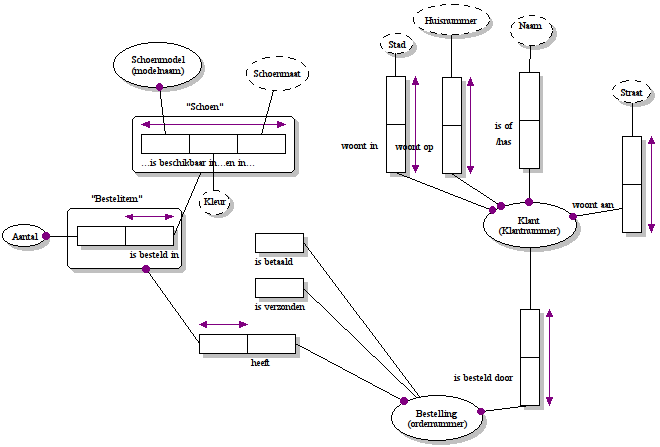
\includegraphics[keepaspectratio=true, width=345pt]{model1.png}
  \caption{ORM Model van het voorbeeldsysteem}
  \label{img:model1}
\end{figure}

\Large{--- Check syntax --- }
\Large{Todo: Fix diagram: Naam, constraint Schoen}

\begin{verbatim}
Schoen: Schoenmodel (modelnaam) is beschikbaar
    in Schoenmaat en is beschikbaar in Kleur.
Bestelitem: Schoen is besteld in aantal.
Bestelling (ordernummer) heeft Bestelitem.
Bestelling (ordernummer) is besteld door 
   Klant (klantnummer).
Bestelling is betaald.
Bestelling is verzonden.
Klant (klantnummer) woont aan 
   Straat (straatnaam).
Klant (klantnummer) woont op 
   Huisnummer (nr).
Klant (klantnummer) woont in Stad (naam).
Klant (klantnummer) heet Naam.
\end{verbatim}

\subsubsection{SQL Tabellen}

Het transformeren van het ORM model naar SQL tabellen is redelijk 
eenvoudig, maar om dubbel voorkomende gegevens te voorkomen heb ik
op verschillende plaatsen een identificatienummer aan tabellen 
toegevoegd als vervangende primary key.

Hier wordt al een duidelijk nadeel van SQL-gebaseerde databases
zichtbaar: het is niet mogelijk om gegevens te objectiviseren.

\begin{table}[htb]
  \centering
  \begin{tabular}{l|l|l|l}
    \textbf{id} & \textbf{Schoenmodel} & \textbf{Kleur} & \textbf{Schoenmaat} \\
    \hline
    1 & Model a              & Zwart          & 43 \\
    2 & Model a              & Zwart          & 42 \\
    3 & Model a              & Wit            & 43 \\
    \ldots & \ldots          & \ldots         & \ldots \\
  \end{tabular}
  \caption{Schoen tabel}
  \label{tab:schoen}
\end{table}

\begin{table}[htb]
  \centering
  \begin{tabular}{l|l|l|l}
    \textbf{id} & \textbf{schoenid} & \textbf{Aantal} \\
    1           & 2                 & 1               \\
    2           & 2                 & 2               \\
    3           & 3                 & 1               \\
    \ldots      & \ldots            & \ldots          \\
  \end{tabular}
  \caption{Bestelitem Tabel}
  \label{tab:bestelitem}
\end{table}

\begin{table}[htb]
  \centering
  \begin{tabular}{l|l|l|l}
    \textbf{Bestelnummer} & \textbf{Bestelddoor} & \textbf{Verzonden} 
    & \textbf{Betaald} \\
    \hline
    1 & 1                &  Y & Y \\
    2 & 1                &  N & Y \\
    3 & 2                & Y  & N \\
    \ldots & \ldots & \ldots & \ldots \\
  \end{tabular}
  \caption{Bestellingen}
  \label{tab:bestellingen}
\end{table}

\begin{table}[htb]
  \centering
  \begin{tabular}{l|l}
    \textbf{Bestelitem} & \textbf{Bestelling}\\ 
    \hline
    1      & 1      \\
    2      & 1      \\
    3      & 2      \\
    \ldots & \ldots \\
  \end{tabular}
  \caption{BestelitemBestelling: Bestelde items horende bij bestellingen}
  \label{tab:bestelitembestelling}
\end{table}

\begin{table}[htb]
  \centering
  \begin{tabular}{l|l|l|l|l}
    \textbf{Klantnummer} & \textbf{Naam} & \textbf{Straat} & \textbf{Huisnummer} & \textbf{Stad} \\
    \hline
    1 & John Doe & Heyendaalseweg & 91 & Nijmegen \\
    2 & Steve Foo & Asselsestraat & 34 & Apeldoorn \\
    3 & Jane Bar  & Kanaalstraat  & 33 & Amsterdam \\
  \end{tabular}
  \caption{Klant tabel}
  \label{tab:klant}
\end{table}

\subsection{Eenvoudige gegevens uit het systeem halen}

\subsubsection{SQL}

Eenvoudige gegevens uit het informatiesysteem halen is eenvoudig in SQL. Een
\verb+SELECT+ statement is erg eenvoudig voor elkaar te krijgen. Bijvoorbeeld
het selecteren van alle verschillende schoenen die in de winkel te koop worden
aangeboden:

\begin{verbatim}
SELECT Schoenmodel, Kleur, Schoenmaat FROM Schoen;
\end{verbatim}

\subsubsection{ORC}

In ORC is het ook eenvoudig om dezelfde gegevens op te halen:

\begin{verbatim}
Schoenmodel, Kleur, Schoenmaat FROM Schoen
\end{verbatim}

Het verschil tussen ORC en SQL is hier niet zo groot. SQL heeft \verb+SELECT+,
ORC heeft \verb+List+, maar verder zou men bijna copy/paste kunnen doen.

\subsection{Conditioneel gegevens uit het systeem halen}

Men wil niet altijd alle gegevens uit een informatiesysteem hebben. Daarom is
het in SQL en in ORC mogelijk om condities op te geven waaraan de op te vragen
informatie moet voldoen.

\subsubsection{SQL}

Stel, ik wil alle verschillende modellen van zwarte schoenen hebben in maat 43.

\begin{verbatim}
SELECT Schoenmodel 
FROM Schoen 
WHERE Schoenmaat = '43' 
  AND Kleur='Zwart';
\end{verbatim}

\subsubsection{ORC}

In ORC gaat het zo: 

\begin{verbatim}
Schoenmodel FROM Schoen in Kleur 'Zwart' 
  AND in Schoenmaat '43'
\end{verbatim}

\end{document}
